As with any high-dimensional optimization problem, the fitter must be vigilant
against the overfitting of data. In practice, this requires:

parsimony with the number of parameters used in the model

common-sense checking "under the hood" of the optimization to verify that
parameter values make sense given the assumptions that undergird the model

understanding of what the value function is (that is, the function being
minimized/maximized) and whether it needs to be changed

cross-correlation between parameters to understand the relationship between
parameters and the effect that each has on predictions made using the model

TCS affected by HF parameters, spin orbit, imaginary above
RCS affected by imaginary above, HF parameters
ECS affected by HF parameters, spin orbit, imaginary above
APower affected by HF parameters, spin orbit,  imaginary above
Charge Density affected by HF parameters, imaginary below
Levels affected by HF parameters, spin orbit,
Spectral functions affected by HF parameters, imaginary below
RMSRadii affected by HF parameters, imaginary below

Physical intuition about scattering data:
- the low-angle ECS/APower data are sensitive to the imaginary strength above
the Fermi surface. The high-angle ECS/APower data are sensitive to the imaginary
strength below the Fermi surface, with the highest angles of elastic scattering
probing the imaginary strength deepest in the core (see high-energy, high-angle
data in Pb)
- the NM correction to the imaginary volume strength is required in all cases to
have the very high/very low energy imaginary strength have the correct trend
(linearly increasing above 100 MeV above, decreasing to 0 below 100 MeV below).
Seen in spectral functions and total cross section data at high energies, where
the pion production channel enters the picture as it goes from virtual->real
- the general trend of the elastic scattering data (not wiggles, but averaged
over wiggles) depends on the imaginary strength at the given energy. If the
minima in the elastic cross sections are too sharp/deep, the imaginary strength
is too large at that energy
- the spin-orbit strength has dramatic effects on the total cross section at low
energies (<20 MeV)
- above the Fermi surface, the imaginary strength is dominated by surface from
0-50 MeV and by volume from 50 MeV up. Below the Fermi surface, the surface
imaginary strength is dependent on A; for low A, where the level density is very
low below the Fermi surface and there's almost no contribution from high LJ
levels, there is virtually no surface imaginary strength below (cf. with charge
density distribution tail, at the surface of the nucleus). As A increases, 
imaginary surface strength below increases gradually but never reaches the
imaginary surface strength above. A consequence of the asymmetry of the
operators that contribute: below 0 MeV, the removal operator LJs
must recouple to the ground state, so high LJ operators have virtually no
contribution; above 0 MeV, addition operators can have arbitrary LJs because
free scattering is possible, adding significantly to the collective strength and
thus is imaginary strength peaked at the surface in the 20-30 MeV range (giant
dipole resonance, for example, surface phonons).

\subsection{Fitting procedure}
The powell method, outlined in Numerical Recipes in C \cite{NumericalRecipes},
was used to minimize the RMS difference between experimental data points and the
values calculated by the DOM. A weighting scheme was assigned to the data points
according to their importance, guiding the fit to reproduce the most essential
data points. From fit to fit, the weighting scheme was adjusted as necessary to
escape local minima in the multidimensional fit.

\begin{figure}
\begin{center}
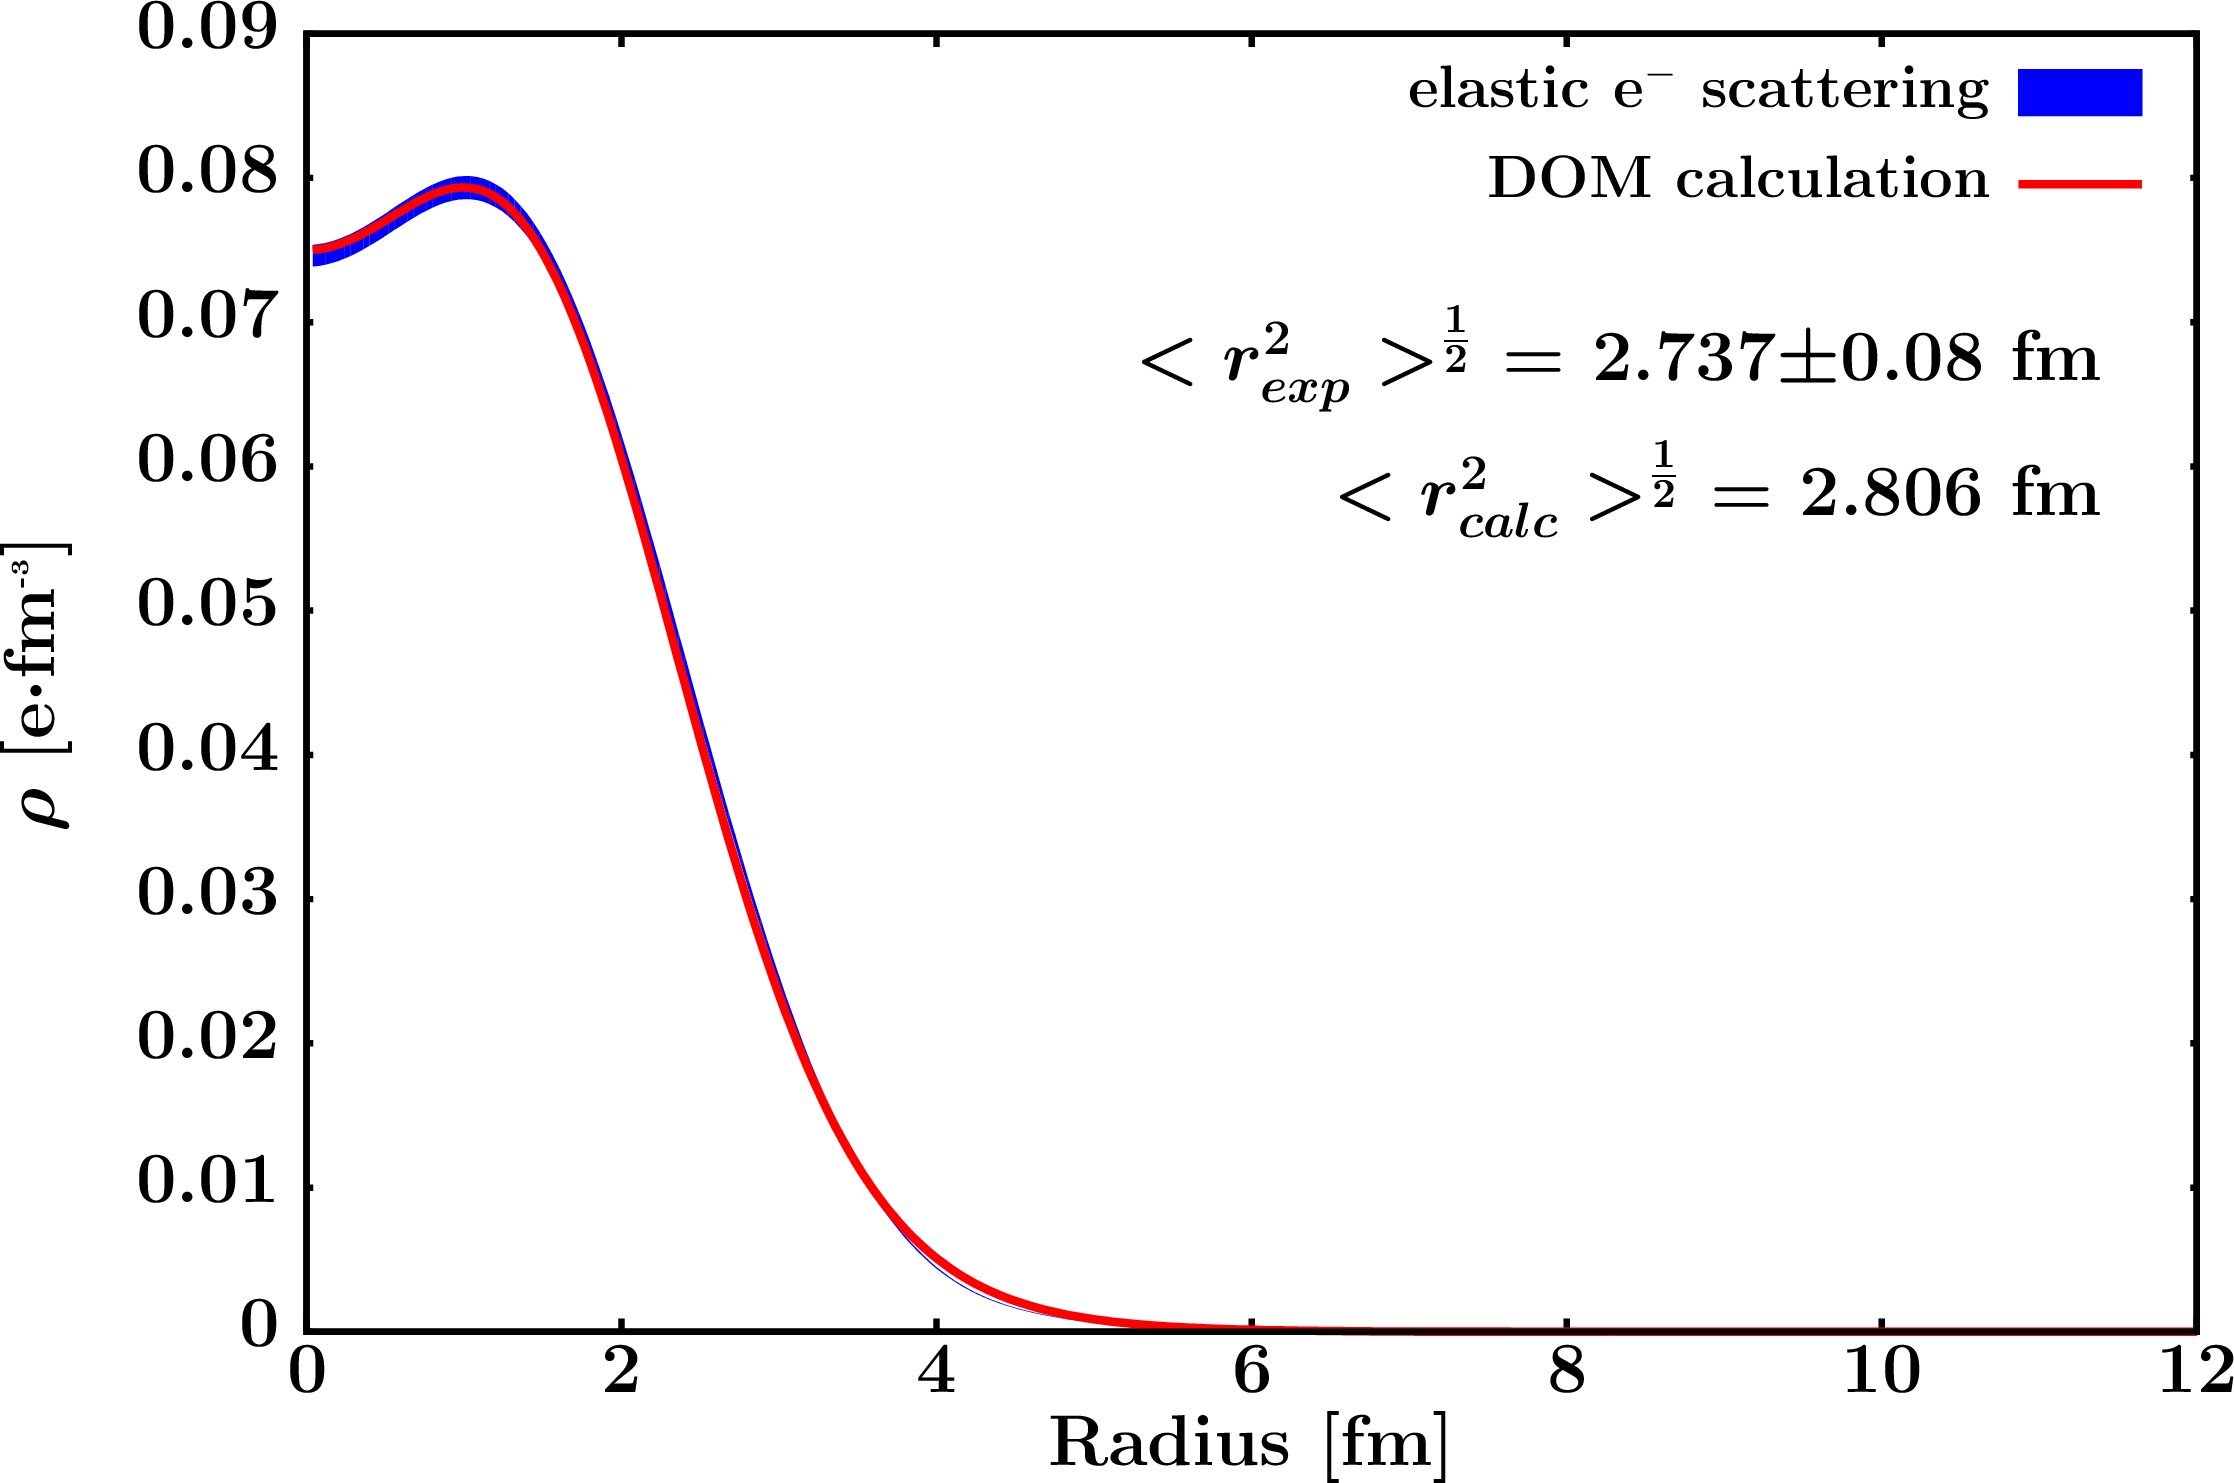
\includegraphics[width = 0.9\textwidth]{figures/o16_chargeDensity.png}
\caption{DOM fit of $^{16}O$ charge density}
\label{o16ChargeDensity}
\end{center}
\end{figure}

\begin{figure}
\begin{center}
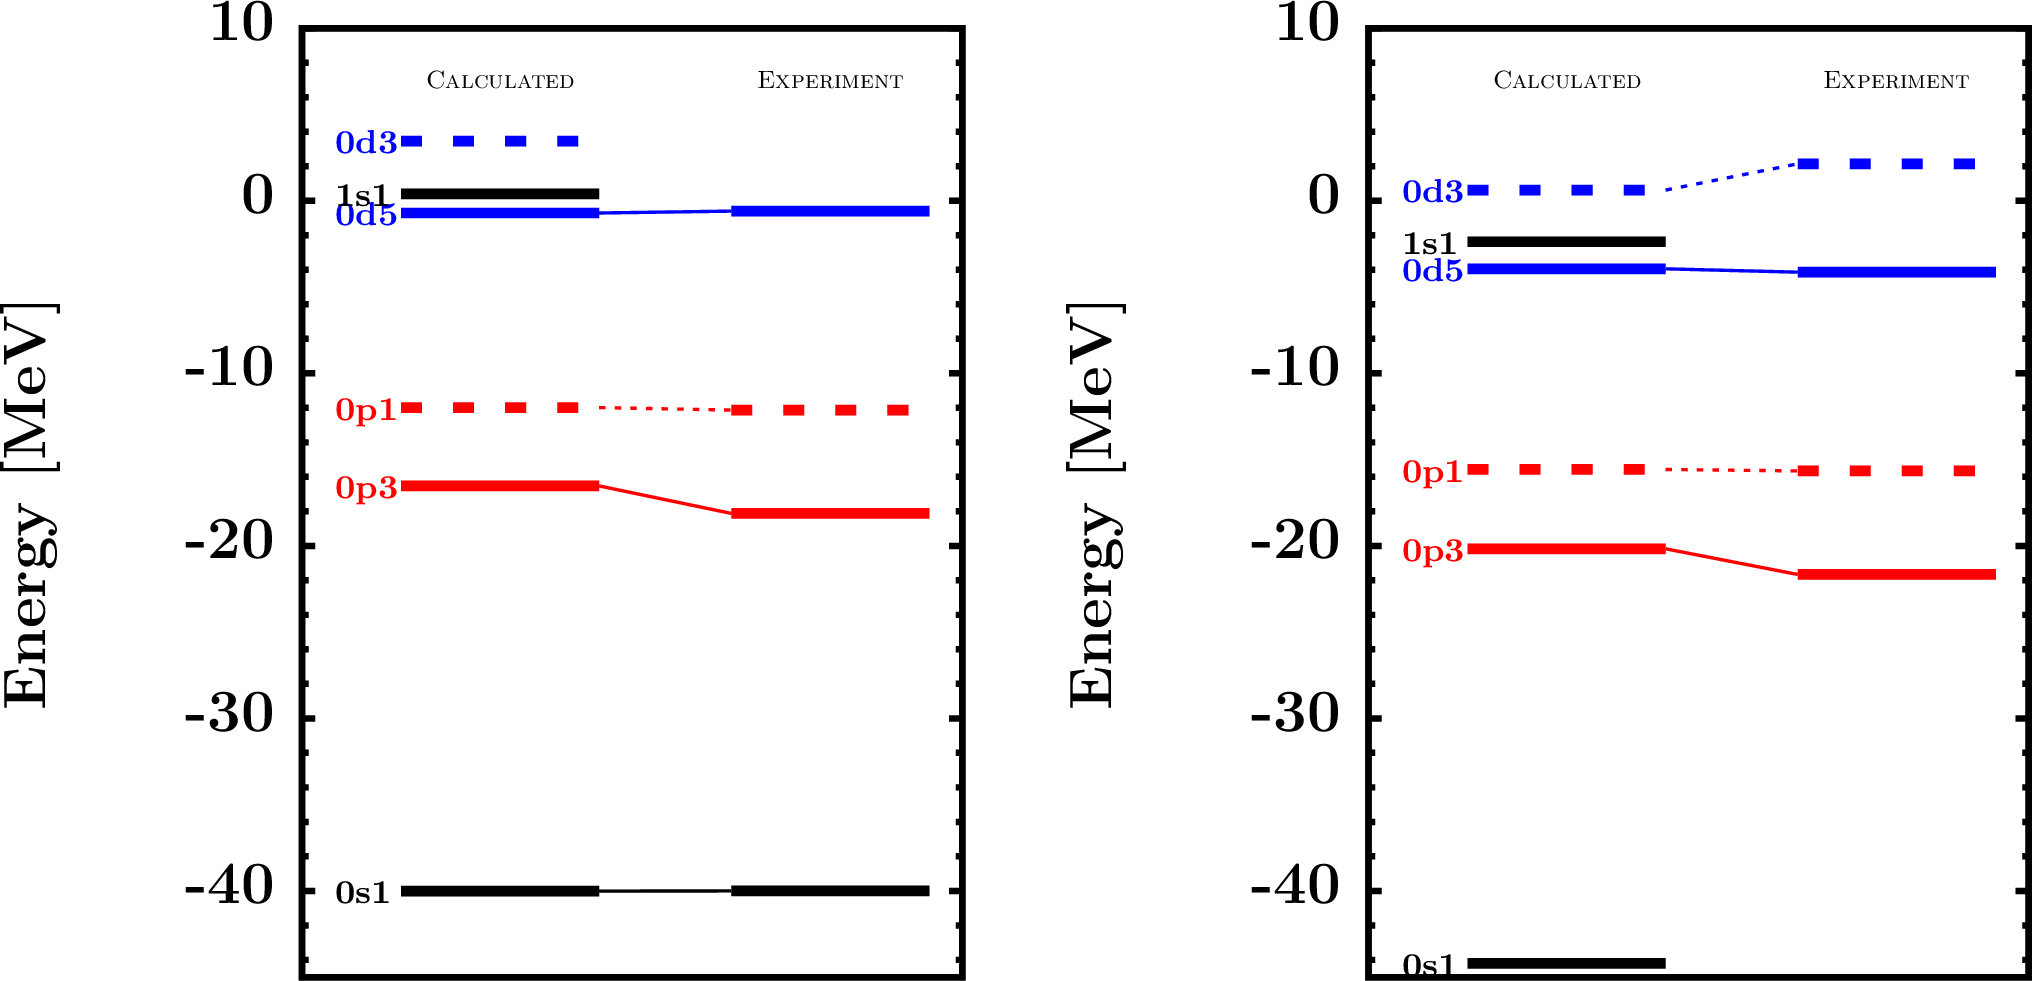
\includegraphics[width = 0.9\textwidth]{figures/o16_SPLevels.png}
\caption{DOM fit of $^{16}O$ single-particle levels}
\label{o16SPLevels}
\end{center}
\end{figure}

\begin{figure}
\begin{center}
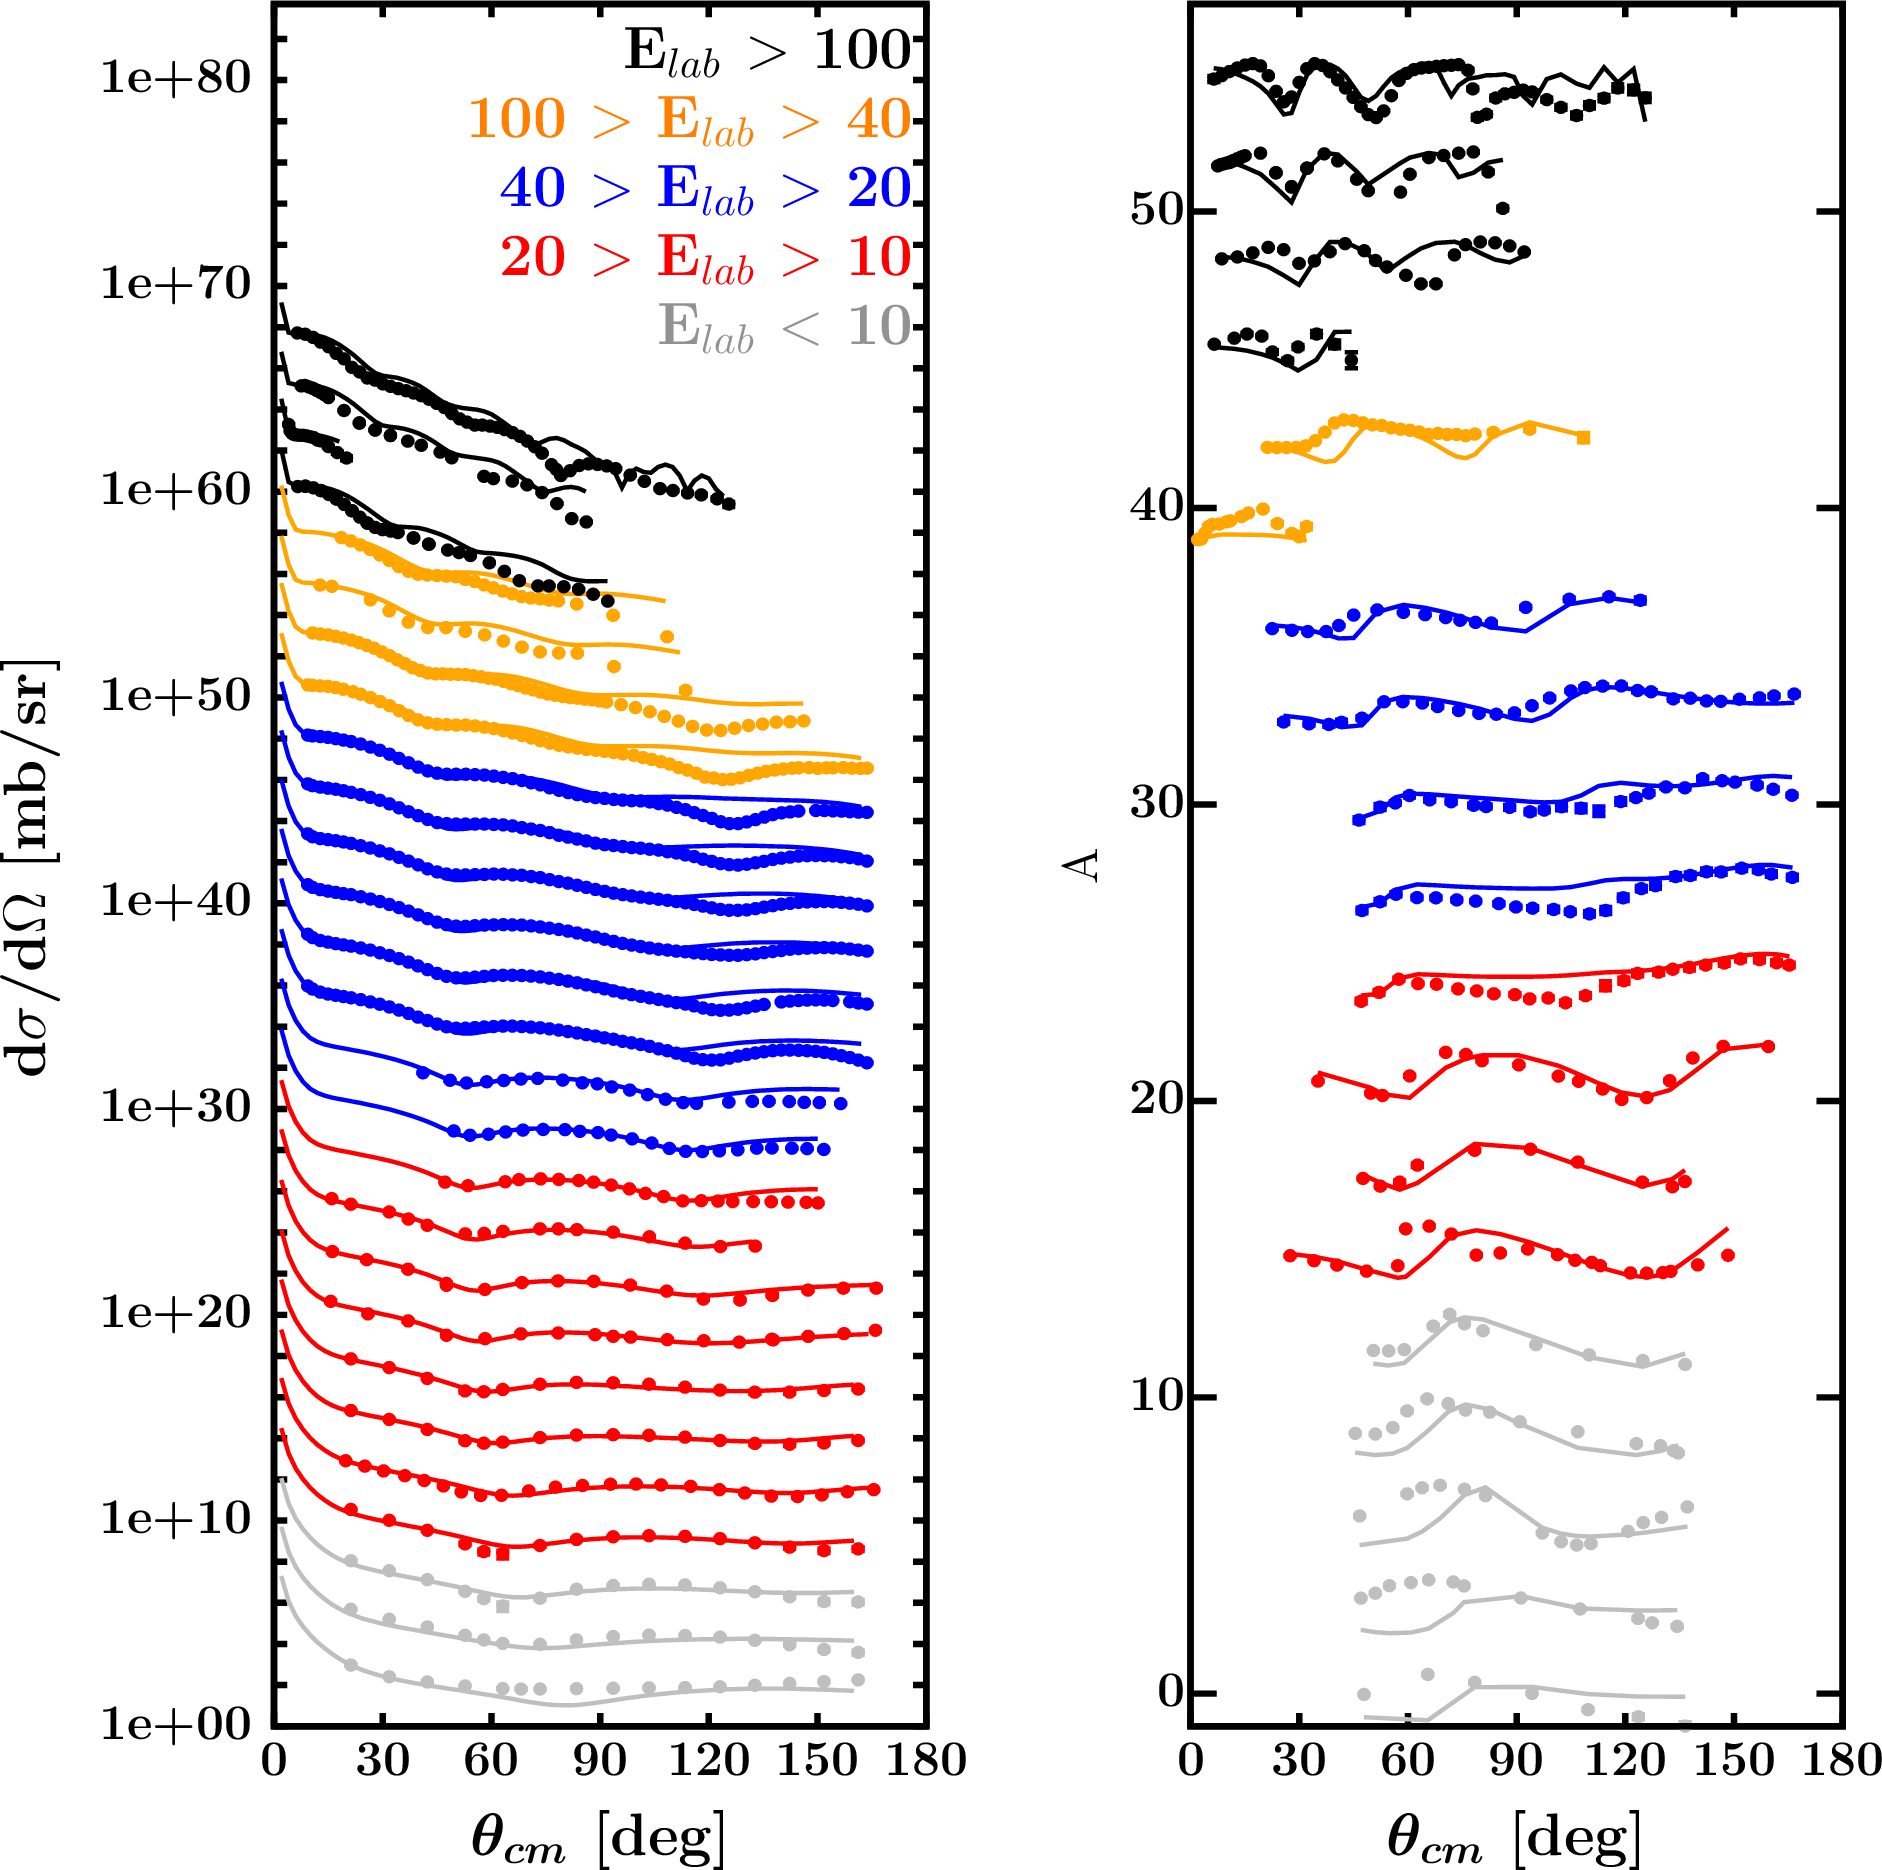
\includegraphics[width = 0.9\textwidth]{figures/o16_protonElastic.png}
\caption{DOM fit of $^{16}O$ proton elastic scattering data}
\label{o16ProtonElastic}
\end{center}
\end{figure}

\begin{figure}
\begin{center}
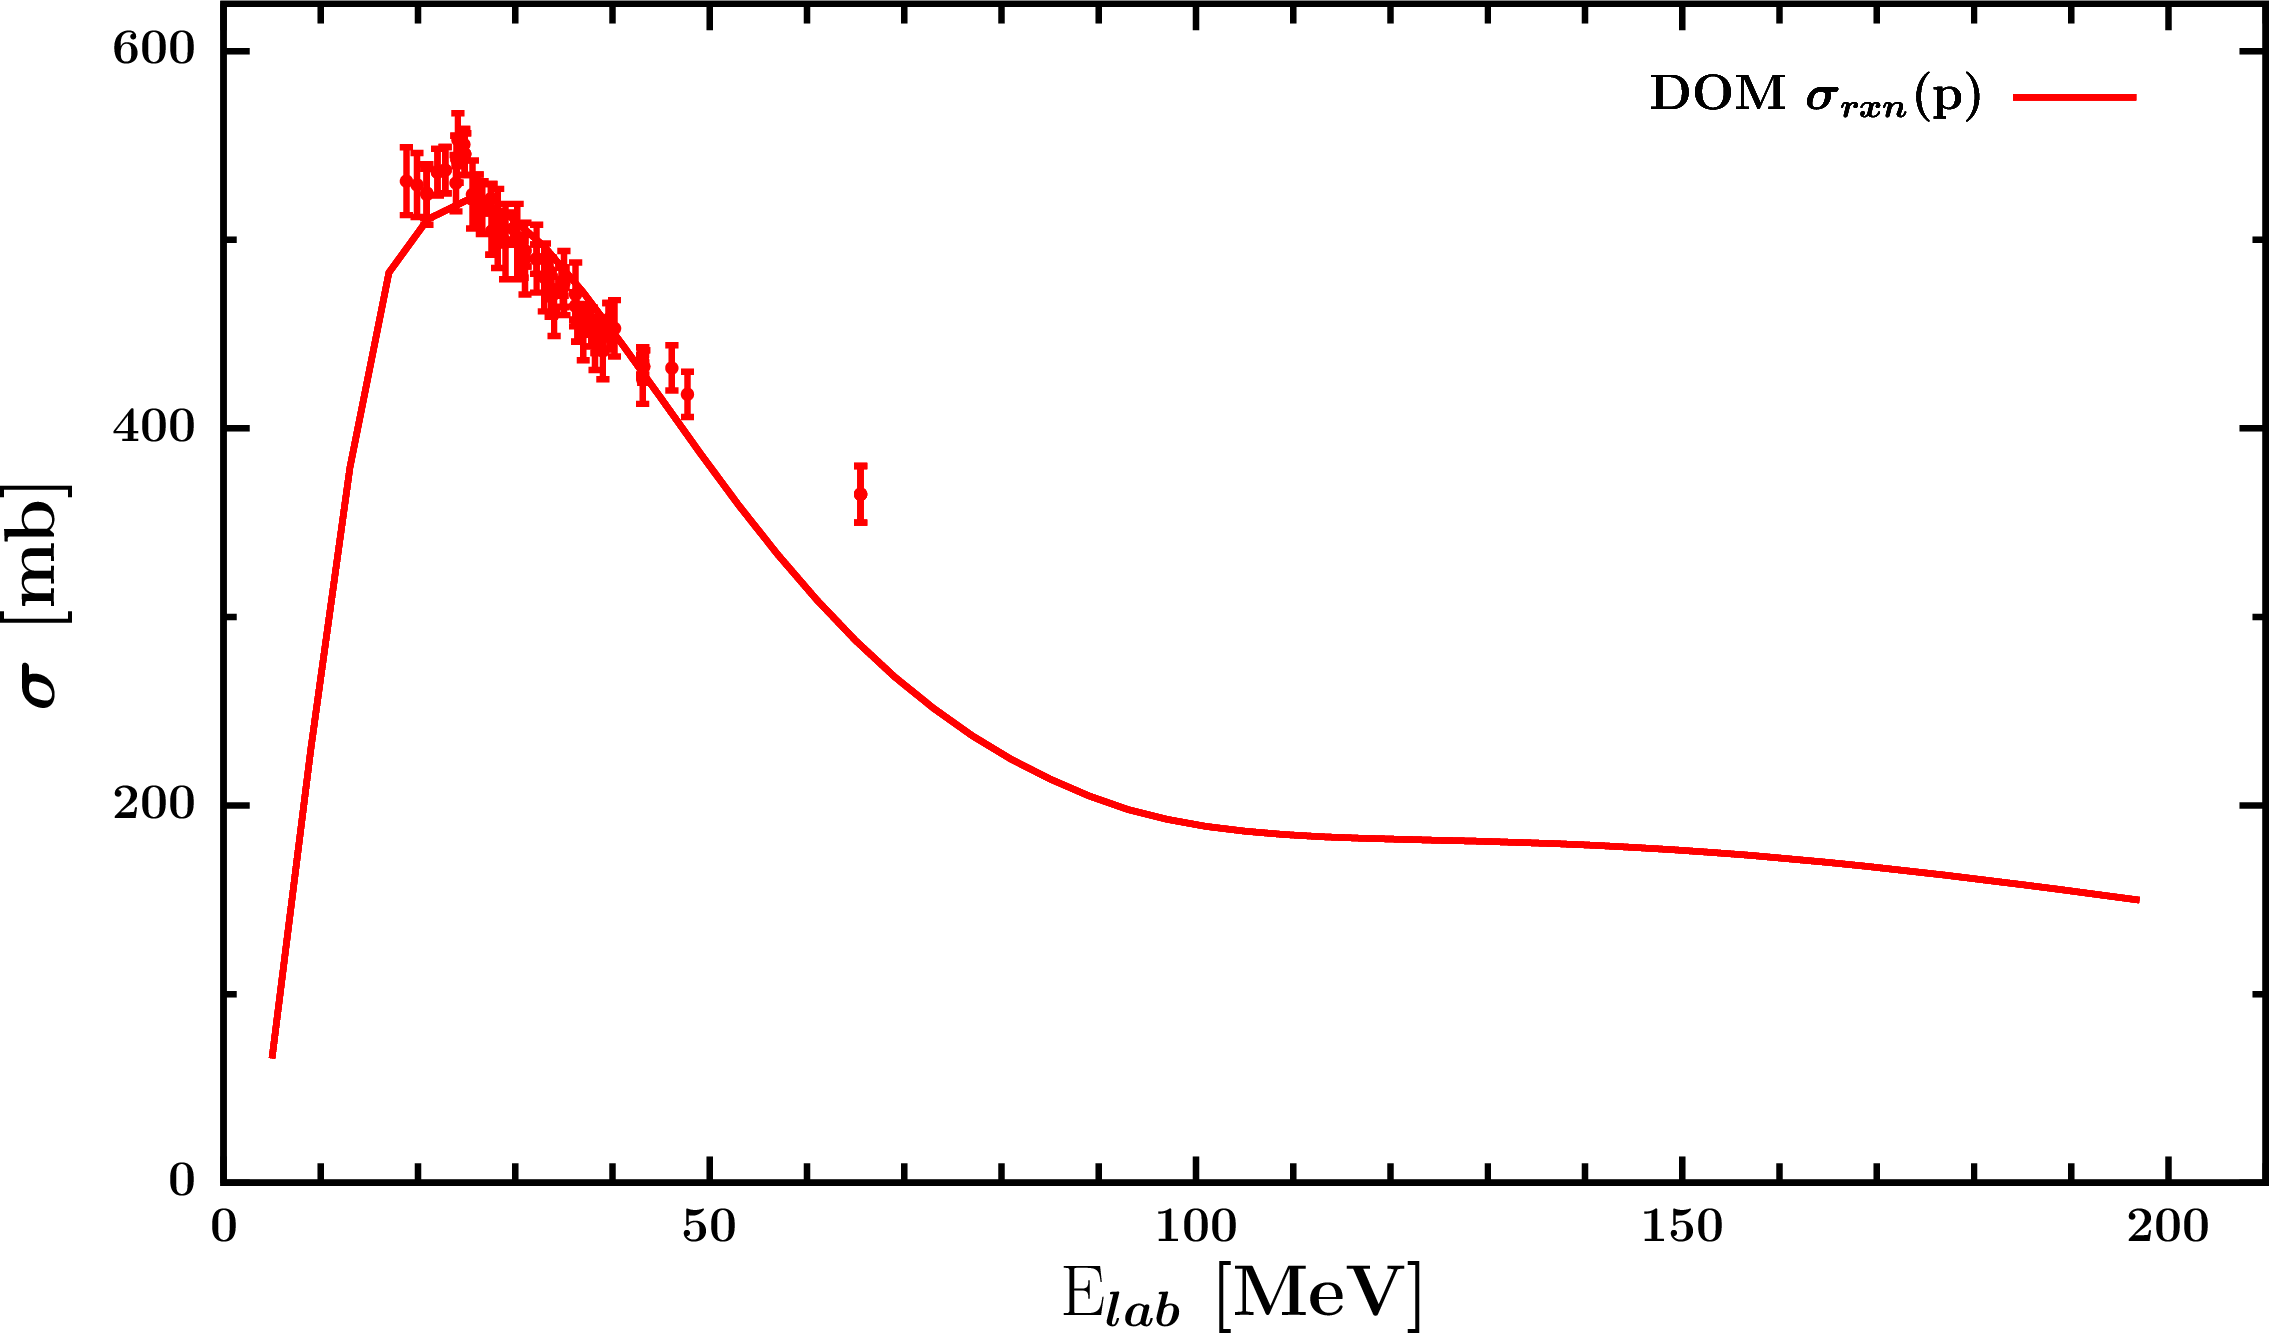
\includegraphics[width = 0.9\textwidth]{figures/o16_protonInelastic.png}
\caption{DOM fit of $^{16}O$ proton inelastic scattering data}
\label{o16ProtonInelastic}
\end{center}
\end{figure}

\begin{figure}
\begin{center}
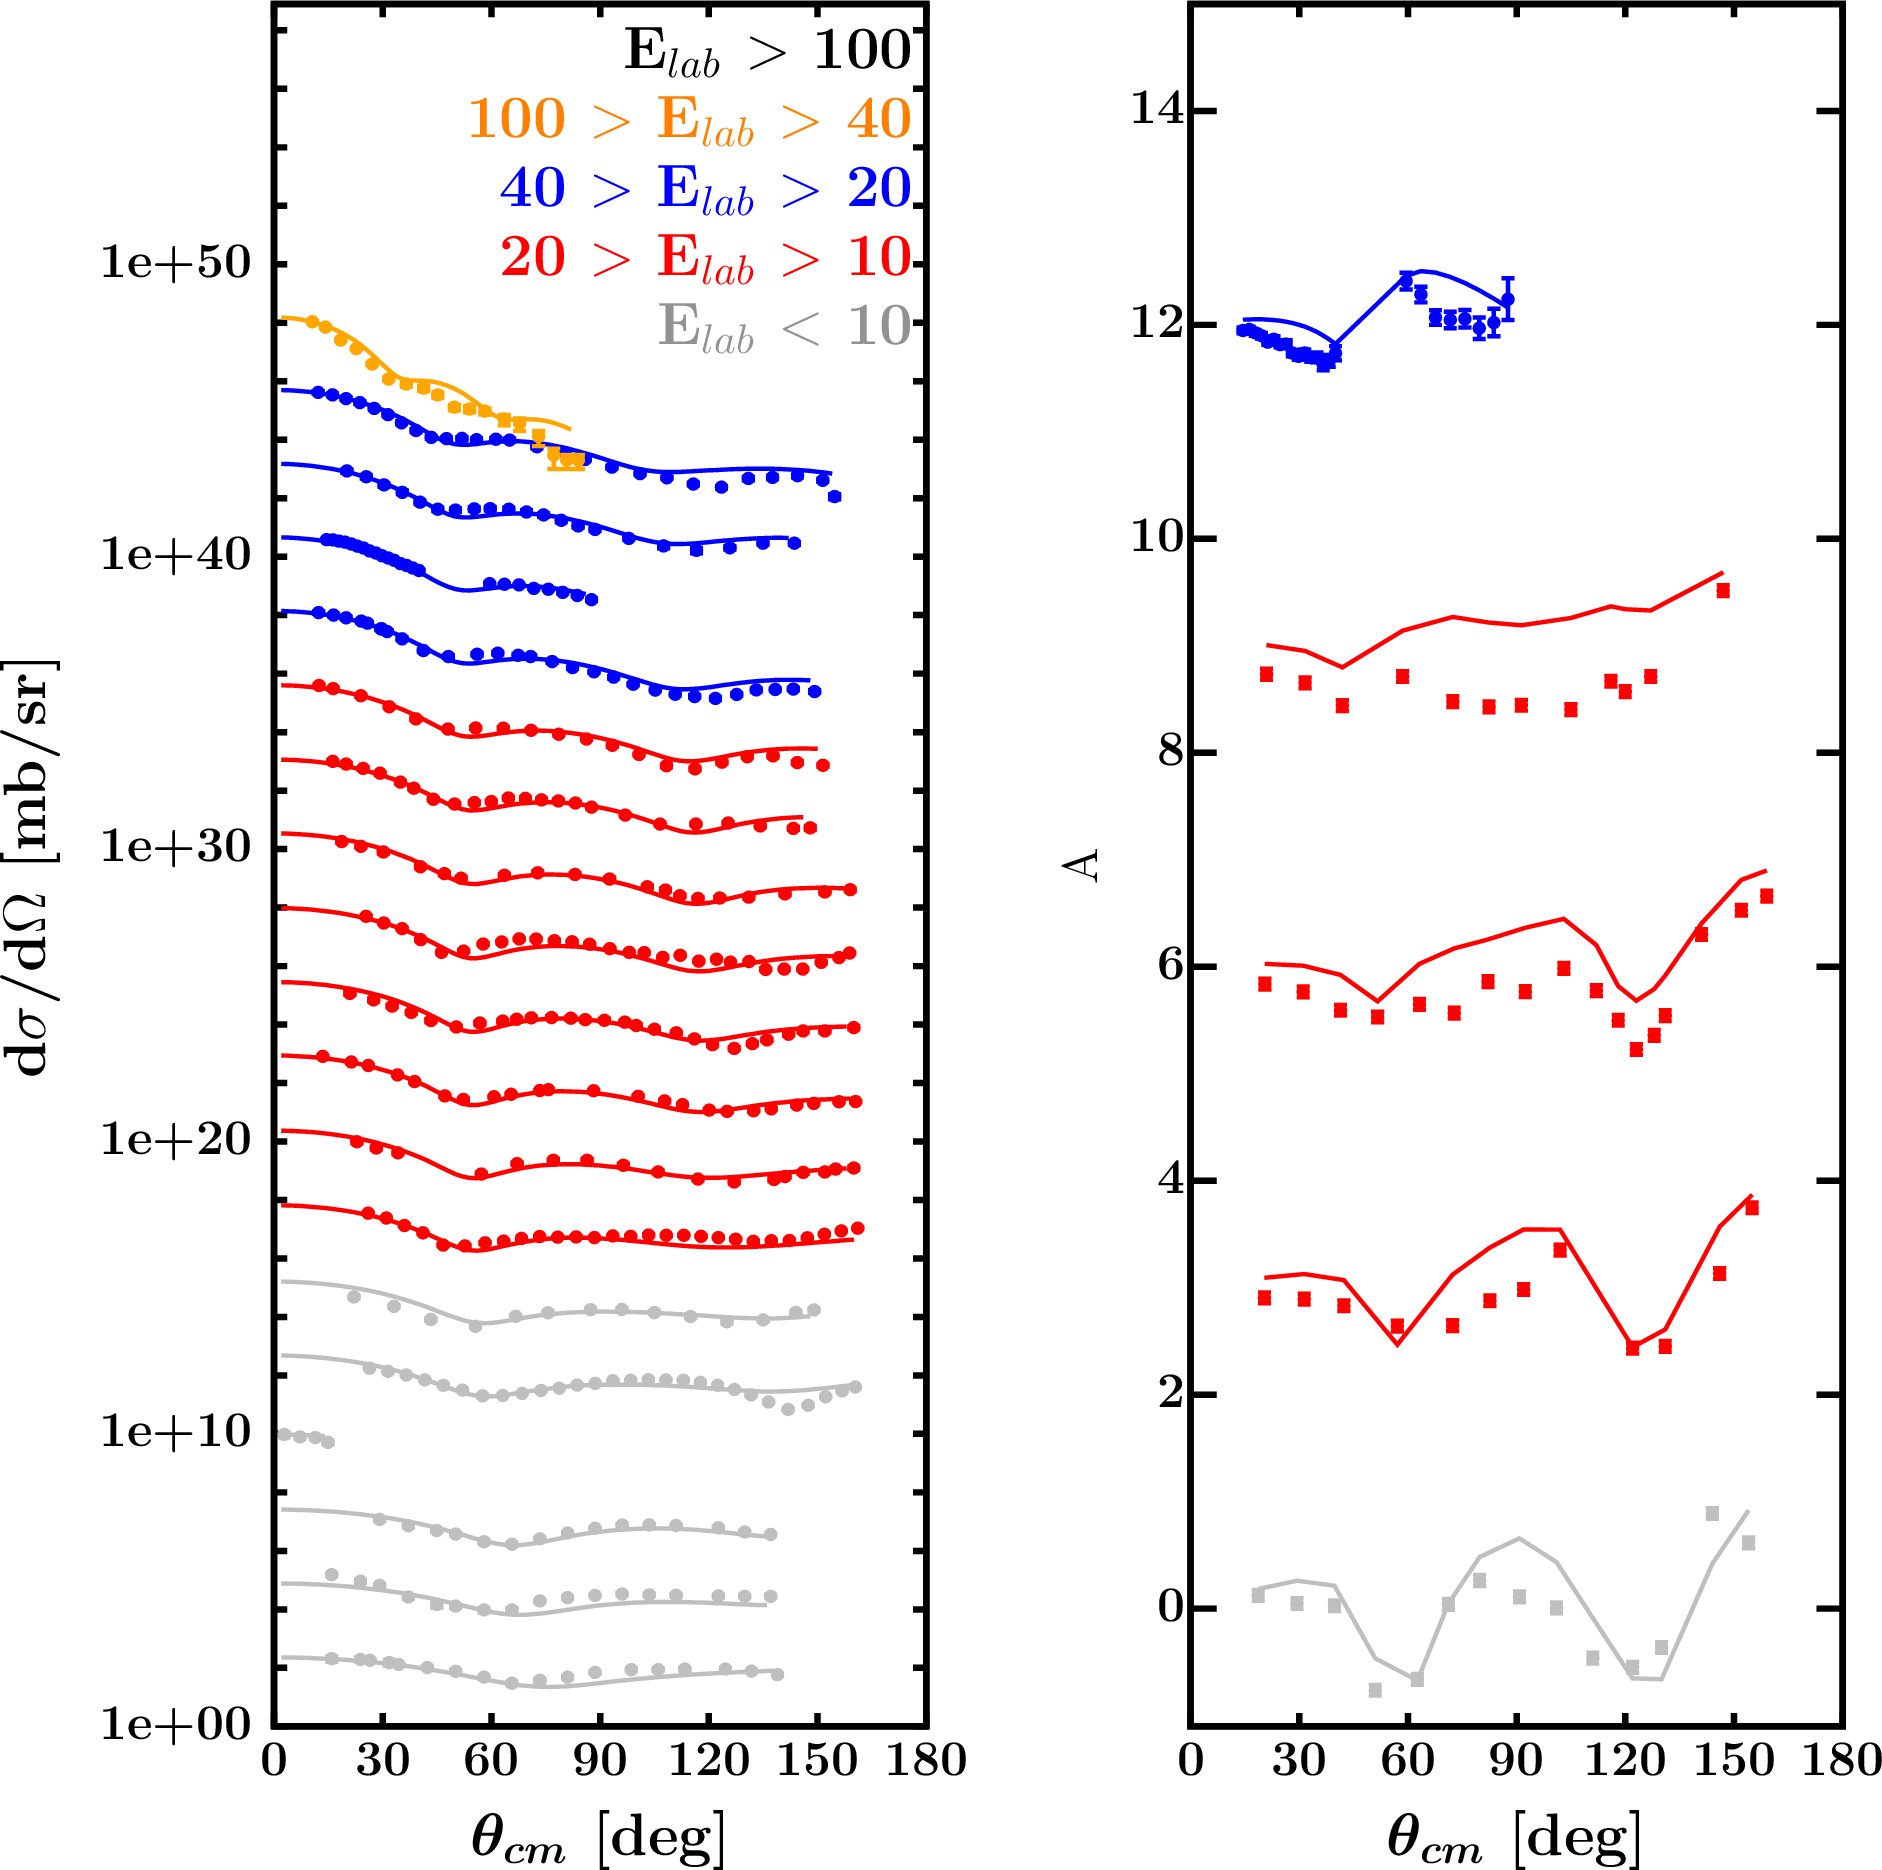
\includegraphics[width = 0.9\textwidth]{figures/o16_neutronElastic.png}
\caption{DOM fit of $^{16}O$ neutron elastic scattering data}
\label{o16NeutronElastic}
\end{center}
\end{figure}

\begin{figure}
\begin{center}
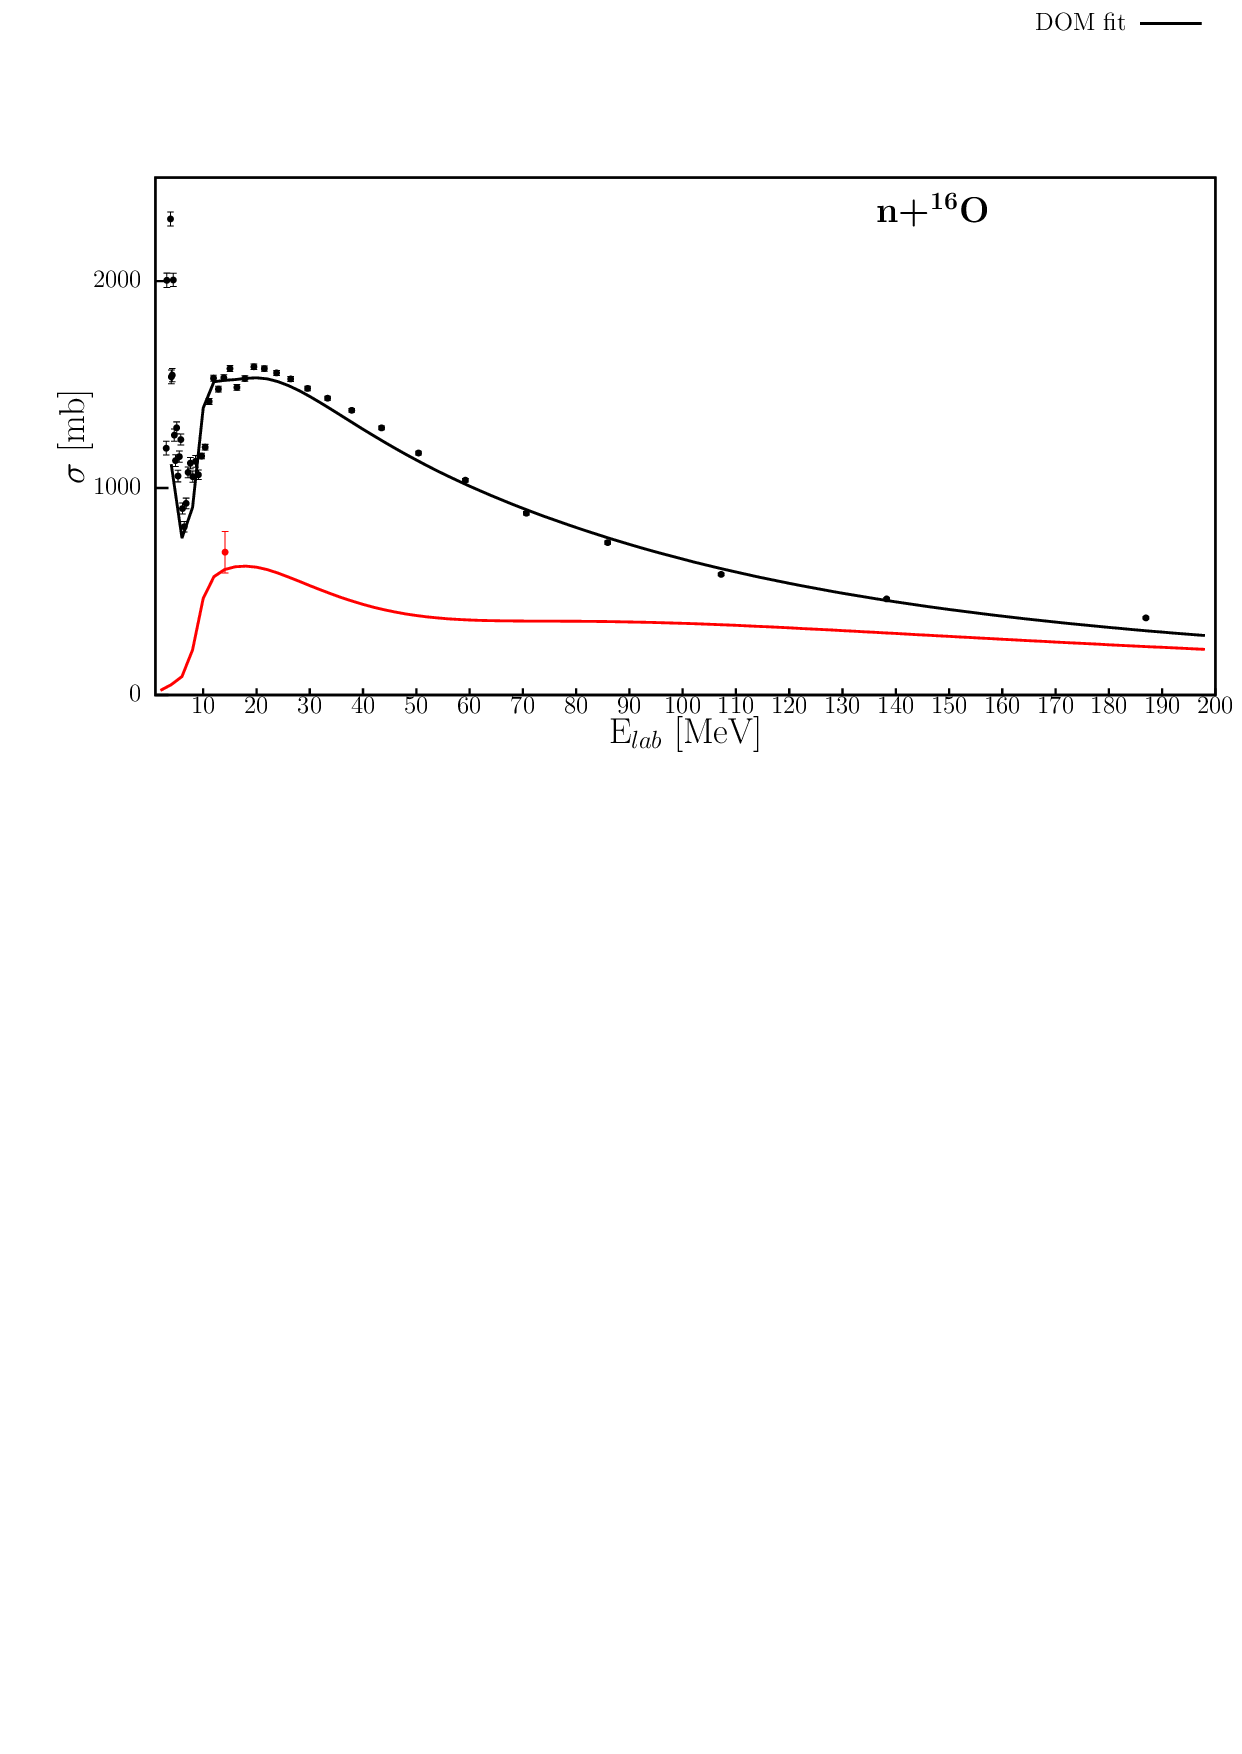
\includegraphics[width = 0.9\textwidth]{figures/o16_neutronInelastic.png}
\caption{DOM fit of $^{16}O$ neutron inelastic scattering data}
\label{o16NeutronInelastic}
\end{center}
\end{figure}

\begin{figure}
\begin{center}
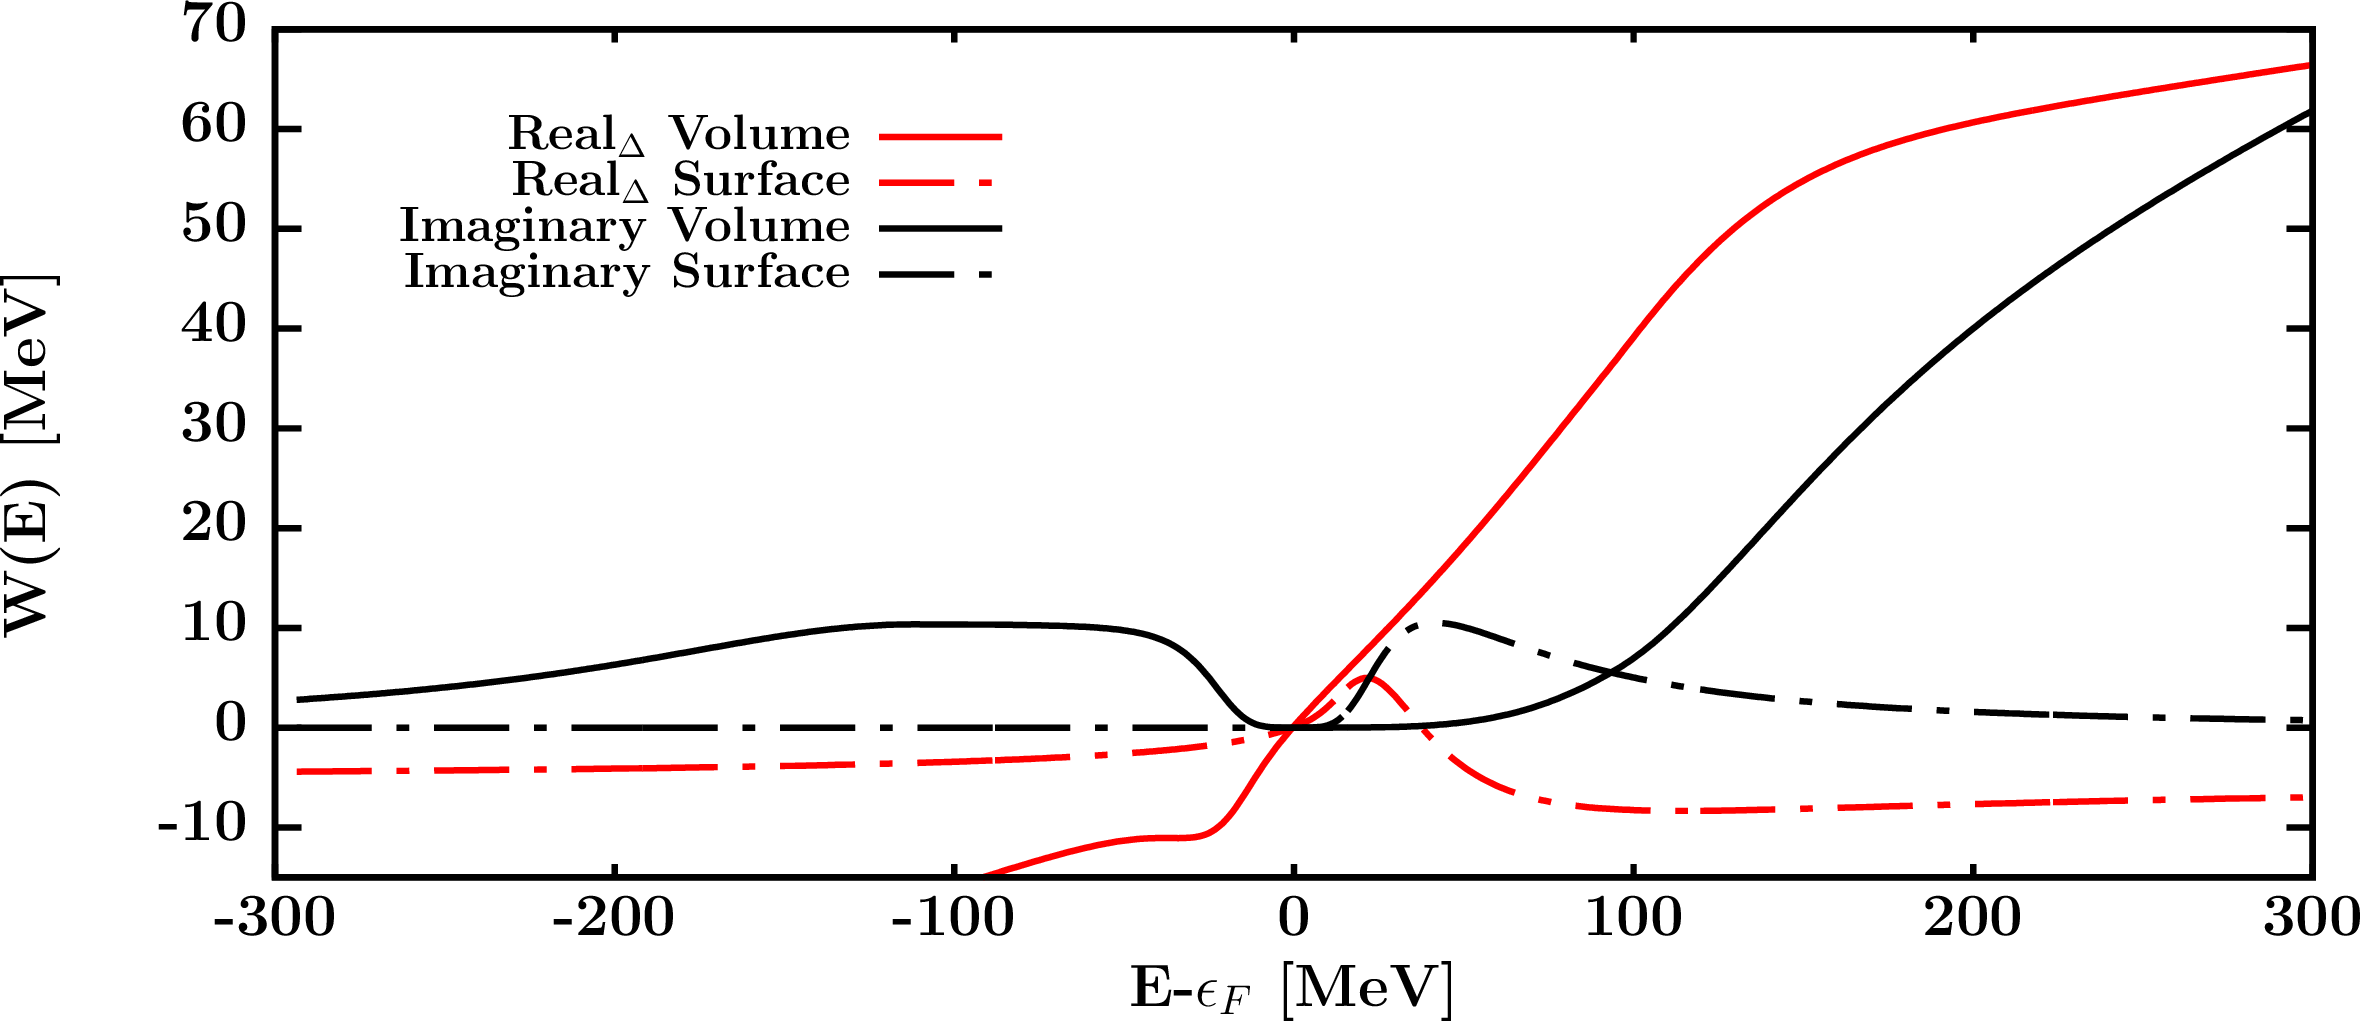
\includegraphics[width = 0.9\textwidth]{figures/o16_protonPotentials.png}
\caption{Visualization of DOM optical potential components for protons on
$^{16}O$}
\label{o16ProtonPotentials}
\end{center}
\end{figure}

\begin{figure}
\begin{center}
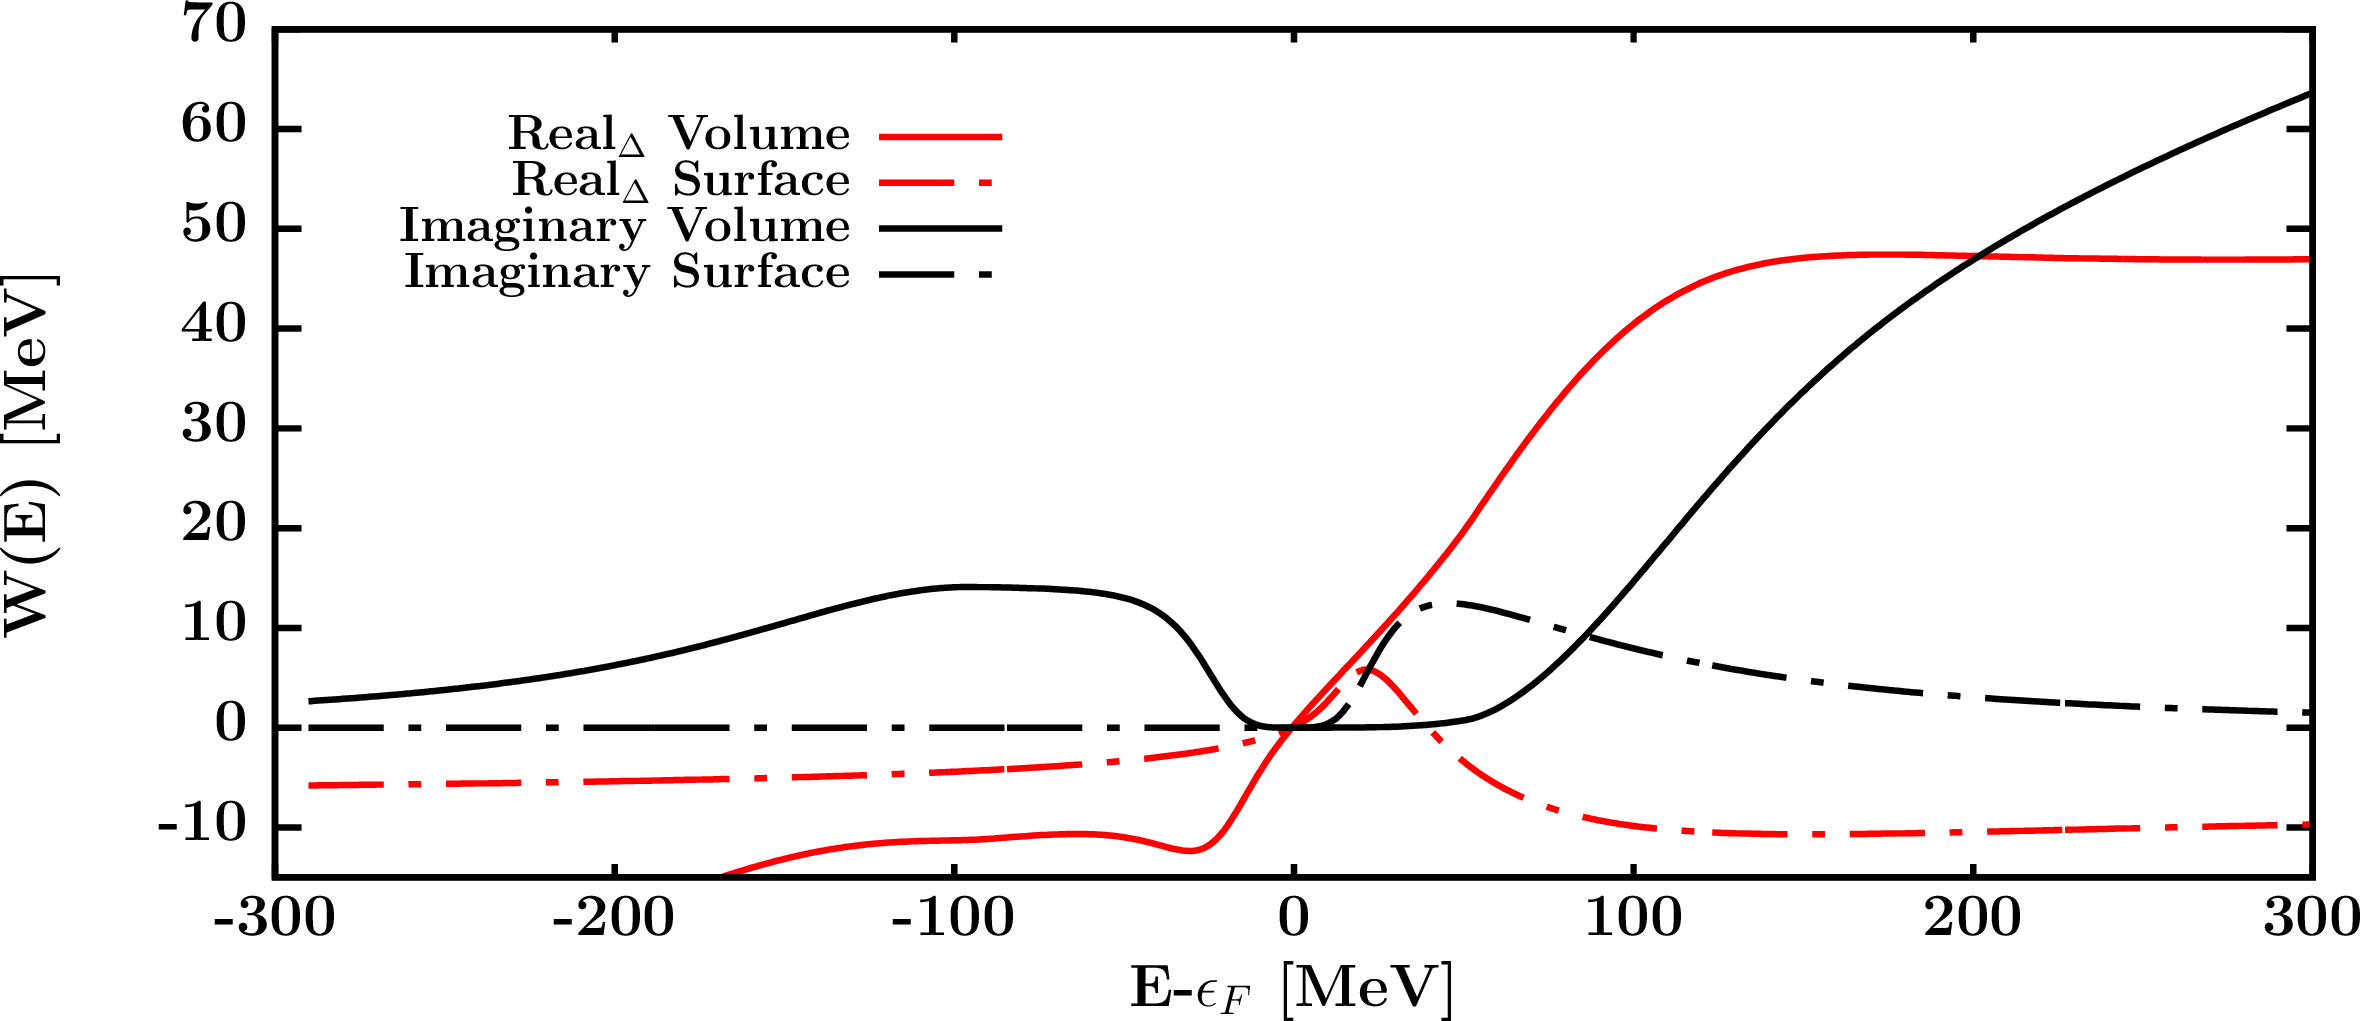
\includegraphics[width = 0.9\textwidth]{figures/o16_neutronPotentials.png}
\caption{Visualization of DOM optical potential components for neutrons on
$^{16}O$}
\label{o16NeutronPotentials}
\end{center}
\end{figure}

\begin{figure}
\begin{center}
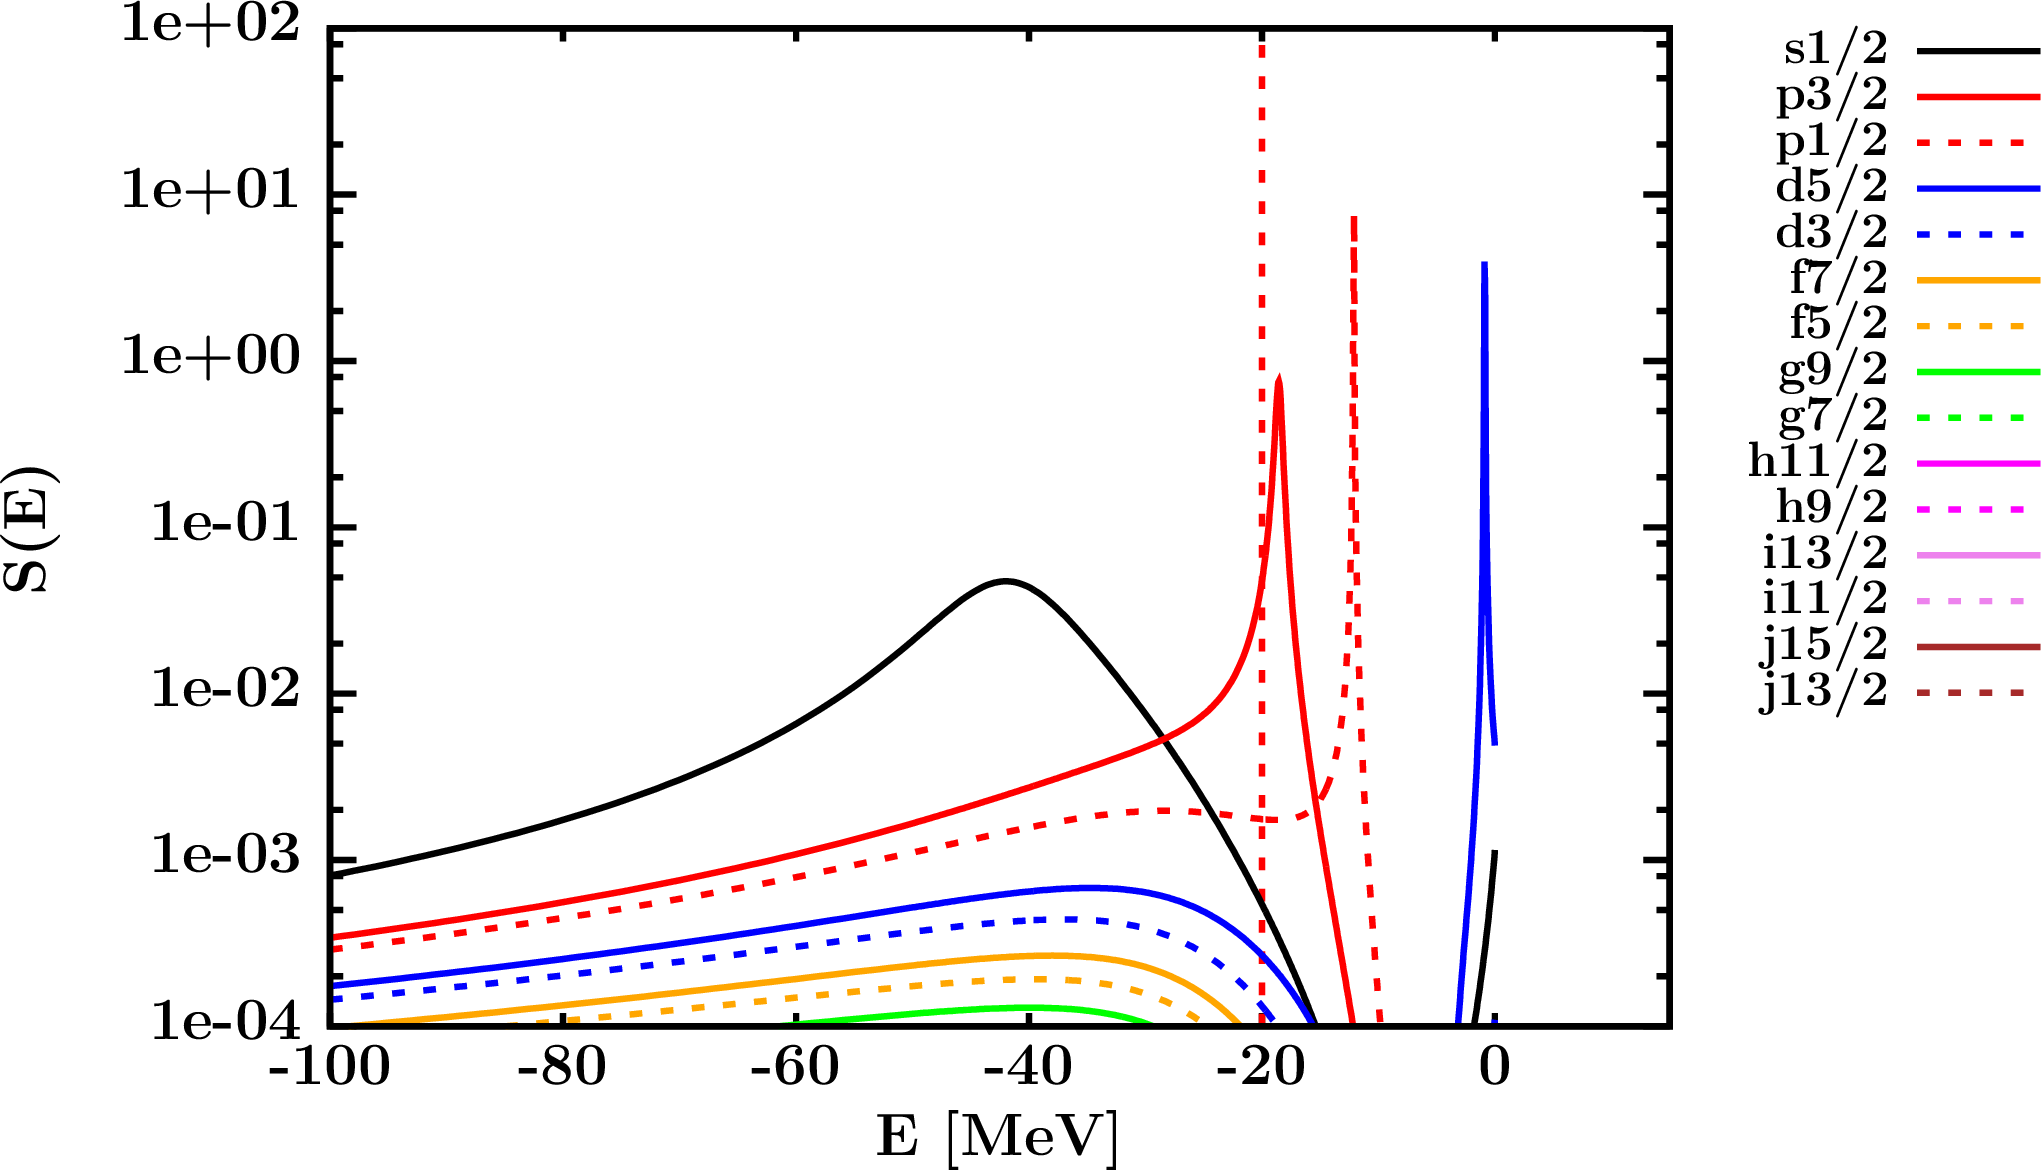
\includegraphics[width = 0.9\textwidth]{figures/o16_protonSpectralFunctions.png}
\caption{DOM calculation of $^{16}O$ proton spectral functions}
\label{o16ProtonSpectralFunctions}
\end{center}
\end{figure}


\begin{figure}
\begin{center}
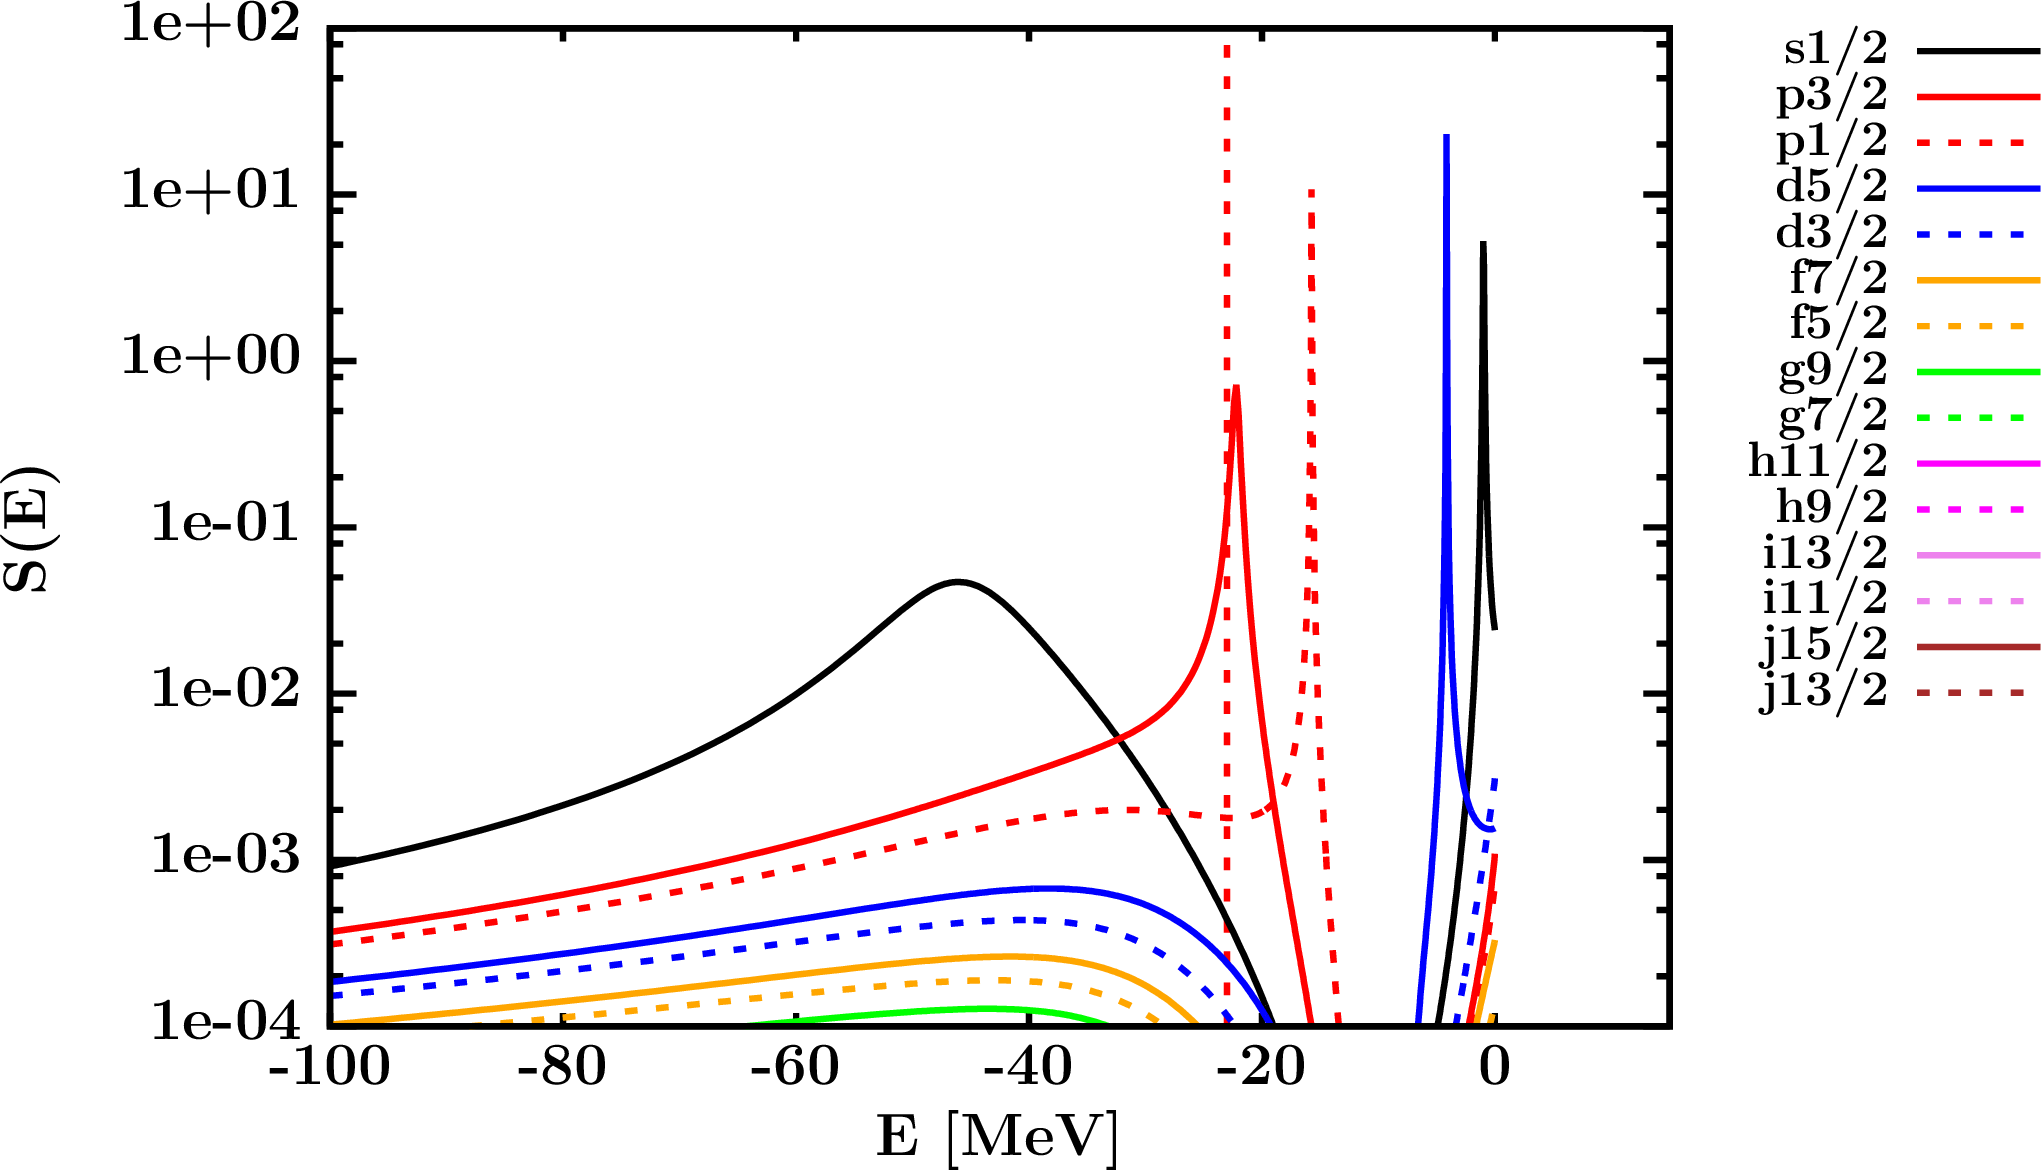
\includegraphics[width = 0.9\textwidth]{figures/o16_neutronSpectralFunctions.png}
\caption{DOM calculation of $^{16}O$ neutron spectral functions}
\label{o16NeutronSpectralFunctions}
\end{center}
\end{figure}

\begin{figure}
\begin{center}
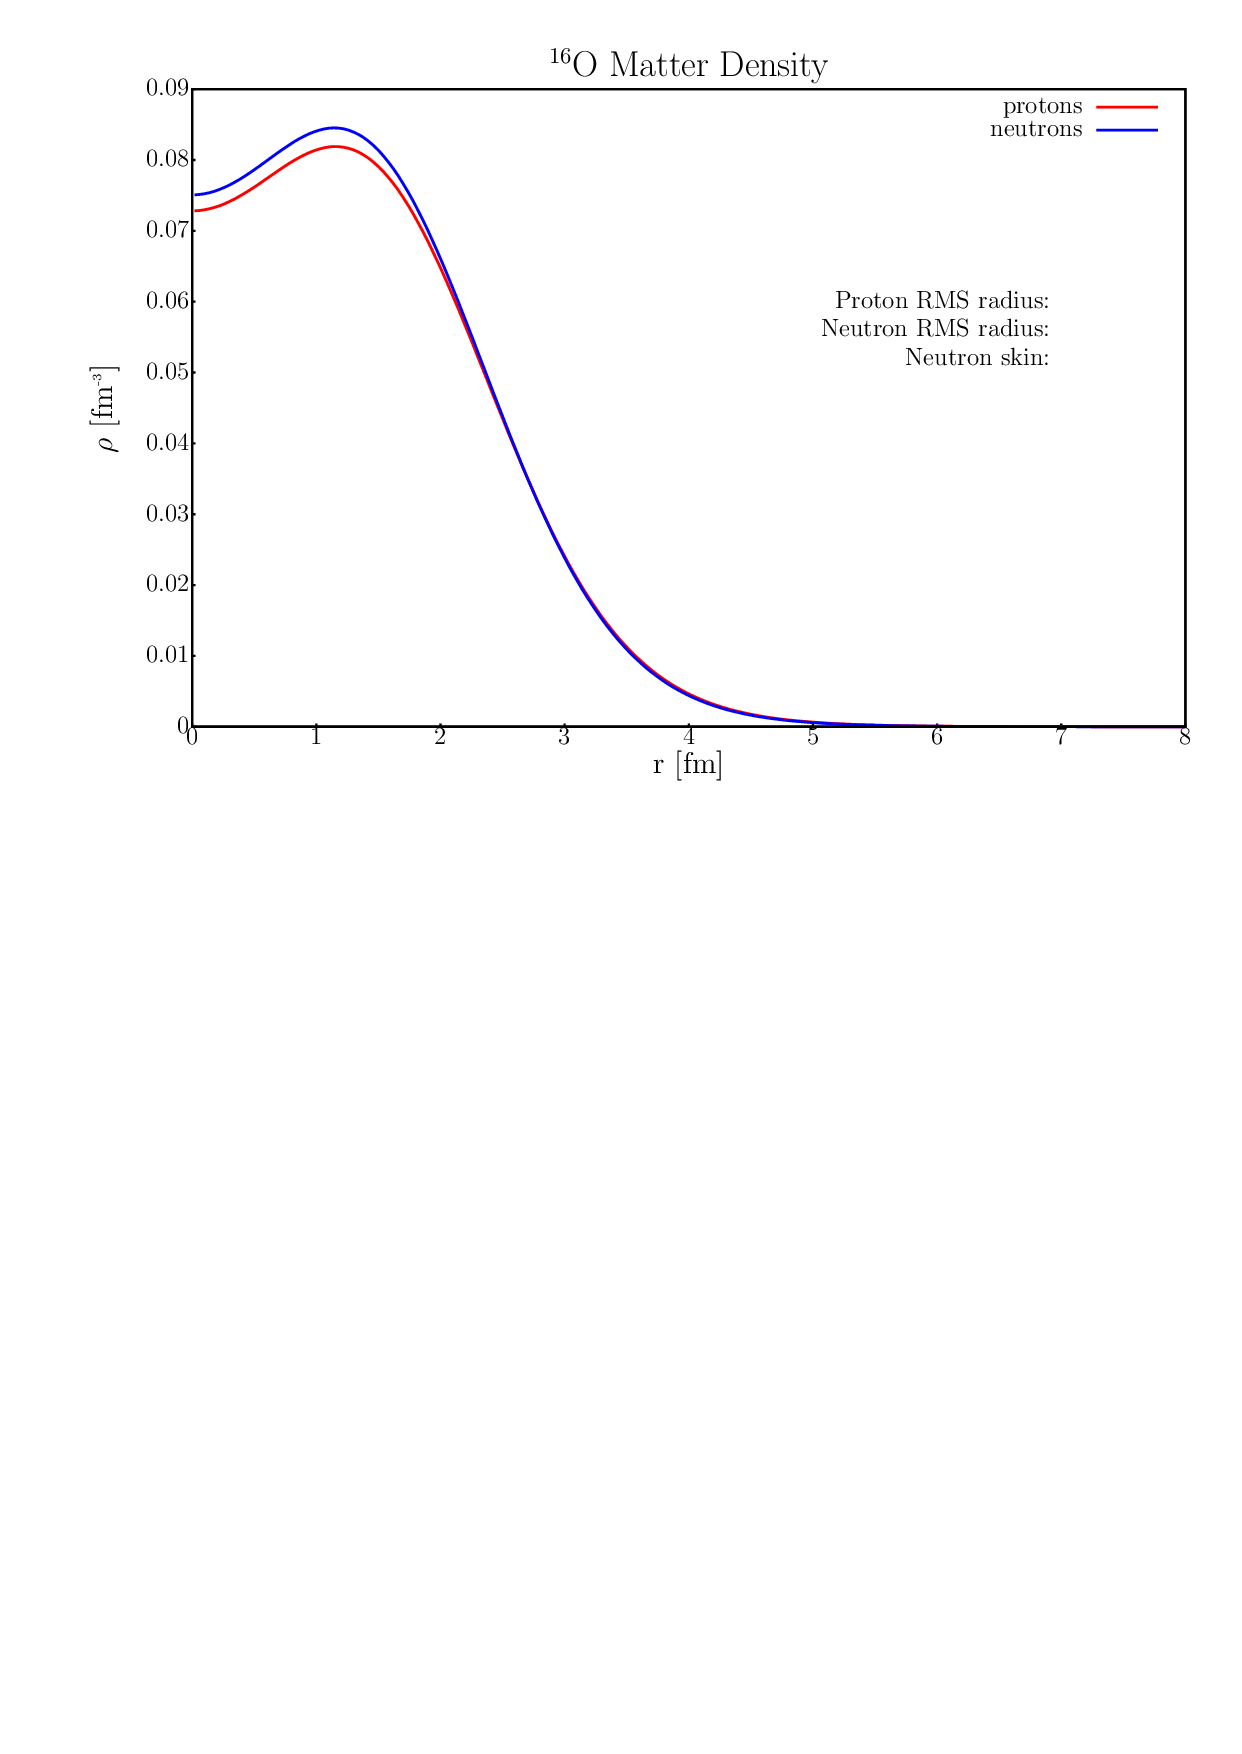
\includegraphics[width = 0.9\textwidth]{figures/o16_matterDensity.png}
\caption{DOM prediction of $^{16}O$ matter density}
\label{o16MatterDensity}
\end{center}
\end{figure}

%\begin{table}
%  \begin{center}
%    \caption{Calibration beams and the energies generated with the degraders.}\label{CBeams}
%  \begin{tabular}{ccccc}
%    \hline \hline
%    Species & Energy & Target & Thickness & Degraded Energy  \\ 
%            & [MeV/A] & &[mg/cm$^2$] & [MeV/A] \\
%     \hline
%    $p$ & 24.2 &  Au & 20.0 & 24.0   \\
%           &  & Al & 429 & 15.8 \\
%    \hline
%    $d$ & 24.2 &  Au &20.0 & 24.1 \\
%            & & Al & 429 &20.3 \\
%    & &  Al & 858 & 15.8 \\
%            & 12.0 &  Au & 20.0 & 11.9 \\
%    \hline
%    $\alpha$ & 24.0 &  Au & 20.0 & 23.8 \\
%     & & Al & 429 &15.6 \\
%    \hline \hline
%  \end{tabular}
%\end{center}
%\end{table}

\afterpage{\clearpage}
